\documentclass{article}
\usepackage[utf8]{inputenc}
\usepackage{macros}

\title{Questions and Answers that somewhat lost relevance}

\begin{document}
\maketitle

\begin{question}
    Is there a relation between the error if $\set{e_1,...,e_k}\subset V$, and the error if $\set{e_1,...,e_k}$ are arbitrary?
\end{question}

\begin{proof}[Answer]\label{A: relationsip between OPT and sample representative error}
We will show that there is such a relationship in the special case when $k=1$ and all vectors in $V$ are of length 1.

Let $S\subset V$, and let $e$ be the principal vector (minimizing sum of square of distances). Let $d(x,y)$ be the distance from $x$ to the projection of $x$ onto $y$ (note that it is not a metric). Let $v\in S$ be the closest vector to $e$, so that $d(v,e)\leq d(w,e)$ for any $w\in S$. We will show that $\sum_{w\in S}d(w,v)^2\leq 4\sum_{w\in S}d(w,e)^2 = 4\text{OPT}$, where OPT = $e_1(S)$ is the optimal (smallest) error.

\begin{lemma}\label{lemma: triangle inequality for projection distance}
For any three unit-length vectors $e,v,w$, we have $d(v,w)^2\leq 2(d(v,e)^2+d(e,w)^2)$, similar to the triangle inequality.
\end{lemma}
Once we prove the lemma we will see that 
\begin{equation}\label{eqn: main equation for proof in case k = 1}
    \sum_{w\in S}d(w,v)^2\leq 2\sum_{w\in S}d(w,v)^2+2\sum_{w\in S}d(v,e)^2\leq 4\sum_{w\in S}d(w,v)^2 = 4\text{OPT}
\end{equation}

We shall now prove the lemma. First, observe that for any two vectors $v,w$ we have $$d(v,w)^2 = \norm{v}^2 - \norm{\proj_w(v)}^2 = \norm{v}^2 - \inp{v}{w}^2/\norm{w}^2$$ by Pythagorean theorem. But $$\norm{v}^2 - \inp{v}{w}^2/\norm{w}^2 = 1 - \cos^2(\gamma) = \sin^2(\gamma),$$ where $\gamma$ is the angle between $v$ and $w$. Let $\alpha$ be the angle between $v$ and $e$, and $\beta$ be the angle between $e$ and $w$. Since we do not care about the direction of vectors here, we may regard the angles between vectors as angles between lines, and restrict all angles to $[0,\pi/2]$. Now observe that $\gamma \leq \alpha + \beta$, meaning $\sin(\gamma)\leq \sin(\alpha+\beta)$, since $\sin$ is increasing on $[0,\pi/2]$. Thus, it suffices to show $\sin^2(\alpha+\beta) \leq 2(\sin^2(\alpha)+\sin^2(\beta))$. In order to see that this is true define $f(\alpha,\beta) = 2(\sin^2(\alpha)+\sin^2(\beta))-\sin^2(\alpha+\beta)$ and minimize it. Taking the gradient of $f$ and equating it to zero, we see that $4\sin(\alpha)\cos(\alpha)=2\sin(\alpha+\beta)\cos(\alpha+\beta) = 4\sin(\beta)\cos(\beta)$, meaning $\sin(2\alpha)=\sin(2\beta)\implies \alpha = \beta$, since we restricted the angles to $[0,\pi/2]$. Thus, minimizing $f$ is equivalent to minimizing $g(\alpha) = 4\sin^2(\alpha)-\sin^2(2\alpha)$. Now note that $g$ is continuous, and by the Intermediate Value Theorem, if it takes negative values (which we want to avoid), there exists $\alpha^*$ with $g(\alpha^*) = 0$. We see that $$g(\alpha^*)=0\iff (2\sin(\alpha^*)-\sin(2\alpha^*))(2\sin(\alpha^*)+\sin(2\alpha^*))=0 \iff 2\sin(\alpha^*)-\sin(2\alpha^*)$$ because $\alpha^*\in [0,\pi/2]$. We see that $\alpha^*=0$ is the only solution to the above, because if $\alpha^*\neq 0$, then $2\sin(\alpha^*)-\sin(2\alpha^*)\iff 2 = \frac{\sin(2\alpha^*)}{\sin(\alpha^*)} = \frac{2\cos(\alpha^*)\sin(\alpha^*)}{\sin(\alpha^*)} = 2\cos(\alpha^*)\implies \alpha^* = 0$, which is a contradiction, since we assumed that $\alpha^* \neq 0$. Therefore, $g\geq0$, and $f\geq 0$, meaning $\sin^2(\alpha+\beta)\leq 2(\sin^2(\alpha)+\sin^2(\beta))$, as required.
\end{proof}

\begin{proof}[Answer from \cite{deshpande2006matrix}]
Theorem $1.4$ of \cite{deshpande2006matrix} states that for any matrix $A$ and $\epsilon>0$, there exist $k+k(k +1)/\epsilon$ rows whose span contains the rows of
a rank-k matrix $\tilde{A}_k$ such that 
$$\norm{A - \tilde{A}_k}^2 \leq (1+\epsilon)\norm{A - A_k}^2 = (1+\epsilon)\opt$$
\end{proof}

\begin{proof}[Alternative proof]
The proof above can be simplified as follows. We will use lemma
\begin{lemma}
For any three unit-length vectors $e,v,w$, we have $d(v,w)^2\leq 4d^2$, where $d = \max\{d(v,e),d(e,w)\}$,
\end{lemma}
which can be proven by squaring the triangle inequality $d(v,w)\leq d(v,e)+d(e,w)$. The triangle inequality holds because distance $d$ is the Hausdorff distance on the Grassmanian manifold $\textbf{Gr(m,1)}$, the $1$-dimensional Grassmanian on $\R^m$. Inequality \ref{eqn: main equation for proof in case k = 1} then becomes 
\begin{equation}
    \sum_{w\in S}d(w,v)^2\leq 4\sum_{w\in S}d_w = 4\sum_{w\in S}d(w,e)^2 = 4\text{OPT},
\end{equation}
where $d_w = \max\{d(v,e),d(e,w)\}$, and $d_w = d(w,e)$, by our choice of $v$.
\end{proof}

\begin{question}
    Is the problem of minimizing $e_1(S)$ equivalent to the problem of maximizing the sum of pairwise dot products $\sum_{v,w\in S}\inp{v}{w}$ ? What about squares of dot products $\sum_{v,w\in S}\inp{v}{w}^2$?
\end{question}

\begin{proof}[Answer]\label{Q: pairwise inner products and rank-1 approximation}
I think maximizing squares of pairwise dot products is equivalent to minimizing $e_1(S)$. The first objective is to maximize $\sum_{v,w\in S}\inp{v}{w}^2$ and the second objective is to maximize $\sum_{v\in S}\inp{v}{e}^2$ for $e$ minimizing $\norm{Ae}$. They certainly look similar.

The answer to the first question is definitely no. Figure \ref{fig: not equivalent} shows an explicit example. But I could not find a counter example to the second question.
\begin{figure}
 \flushright
 \caption{\label{fig: not equivalent}}
 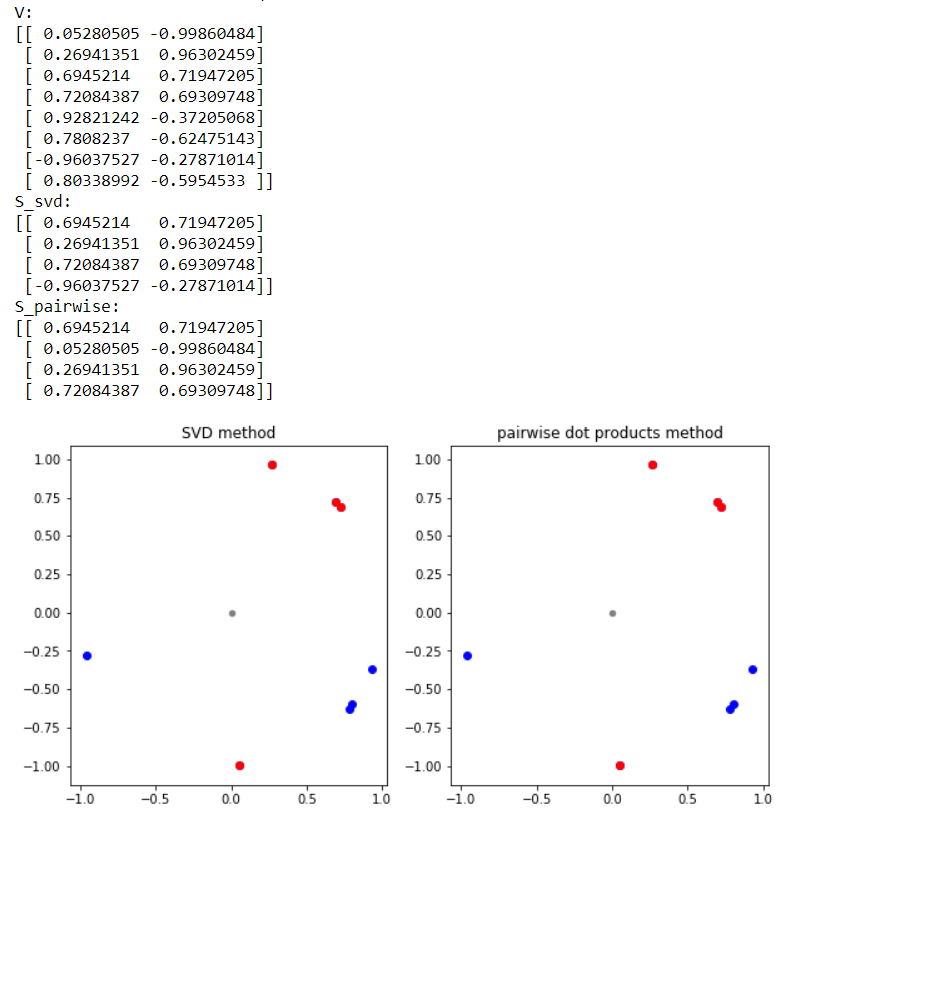
\includegraphics[width=0.5\textwidth]{images/not_equivalent.png}
\end{figure}
\end{proof}

\begin{question}
We want to find $S\subset V$ of size $n$ and $E\subset \R^m$ to maximize $$\sum_{w\in S}\norm{\proj_{\vspan{E}}(w)}^2.$$
    
If $E$ is given, can find $S$ easily (iterating through all $v\in V$ and choosing $n-k$ of them with biggest length of projection onto $\proj_{\vspan{E}}$). If $S$ is given, can approximately find $E$ (SVD). What about both at the same time? Some kind of analogue of $EM$, perhaps?
\end{question}

\begin{proof}[Answer]
Here is an algorithm similar to $EM$.
\begin{algorithm}[H]
\caption{FindEandS}
\label{alg: EM-like alg}
    \begin{algorithmic}[1]
    \State Pick random $E\subset \R^m$ by picking each coordinate of $e_i$ uniformly at random from $[-1,1]$, and normalizing each $e_i$. We can Gram-Schmidt $E$ but it's not necessary.
    \While{true}:
        \State Find $S$ for $E$ (by iterating through all $V$ and checking $d(v,\vspan{E})$)
        \State Find $E$ for this $S$ (via SVD)
    \EndWhile
    \textbf{return} $S,E$.
    \end{algorithmic}
\end{algorithm}
\textbf{Are there any guarantees on this?}
\end{proof}

\begin{question}[Similar Problem]
    Projective clustering is the problem of finding a set of $j$ $k$-dimensional subspaces $F_1,...,F_j$ such that $$\sum_{p\in P}\min_i d(p,F_i)$$
    for a set of points $P\subset \R^m$. This is known to be \textbf{NP}-hard \cite{deshpande2006matrix}. The subspaces partition $P$ into parts $P_1,...,P_j$, where $P_i$ is the set of points closest to $F_i$. If $P_i$'s were required to be of a specific size (e.g. all of them of size $n$), then solving problem \ref{Q: geometric question} $N/n$ times would solve the modified projective clustering problem. Thus, most likely, problem \ref{Q: geometric question} is \textbf{NP}-hard.
\end{question}

\begin{question}[Basic SVD questions]\label{Q: SVD questions}
    Given matrix $A = (a_1,...,a_n)$ and its $k-$approximation $A_k$ with (left) principal vectors $E = e_1,\dots,e_k$, is $\norm{A - A_k} = \sum_{i\leq n}\norm{a_i - \proj_{\vspan{E}}(a_i)}^2$? Is $e_1 = \frac{1}{n}\sum_{i\leq n}a_i$? Note that $\proj_{\vspan{E}}(a_i) = \sum_{j\leq k}\inp{a_i}{e_j}$.
\end{question}
\begin{proof}[Answer to \ref{Q: SVD questions}]
The answer to the first question above is ``yes". Let's consider the case when $A$ is mean-centered (mean of each row is 0), in which case $e_1 \neq \frac{1}{n}\sum_{i\leq n}a_i = 0$. First, consider $k=1$. For a given $i$, $\norm{a_i - e_1\inp{a_i}{e_1}}^2 = \norm{a_i}^2 - \inp{a_i}{e_1}^2$ (just algebra). So $\sum_{i\leq n}\norm{a_i - e_1\inp{a_i}{e_1}}^2 = \sum_{i\leq n}\norm{a_i}^2 - \inp{a_i}{e_1}^2 = \norm{A}^2-\sum_{i\leq n}\inp{a_i}{e_1}^2$. We know that $e_1$ maximizes variance in the direction $e_1$, which is given by $\sum_{i\leq n} \inp{a_i}{e_1}^2$, meaning $e_1$ minimizes $\sum_{i\leq n}\norm{a_i - e_1\inp{a_i}{e_1}}^2$. I think the rest ($k>1$) follows by induction (define the new $A$ to be $A-A_1$).

The answer to the second question is ``no"! For the case when A is not mean-centered, I produced an explicit counter-example (generated a random matrix and tried it). For the case when A is mean-centered, $\frac{1}{n}\sum_{i\leq n}a_i = 0$, and so cannot equal $e_1$, since $e_1$ is non-zero. Here is a specific example: let $A = \Big((-1,k),(1,k)\Big)^T$. Note that the mean of the two vectors is $\mu=(0,k)$. If $k>1$, the first principal vector is $(0,1) = \mu/\norm{\mu}$. But if $k<1$, the first principal vector is $(1,0)$, orthogonal to the mean $\mu=(0,k)$. If $k=1$, both principal vectors have equal singular values.
\end{proof}
\begin{question}
    What happens to the low-rank approximation of a matrix when I replace one vector by another?
\end{question}

\section{Research Summary}
Evimaria Terzi and I, Vasily Ilin, are interested in detecting dense low-rank subgraphs. 
The setup is as follows: we are given a graph G = (V,E), where V is a subset of m-dimensional Eucludean space $\R^m$. Given a subset S of V, one can ask for the "effective rank" of the matrix A spanned by S (matrix rows are given by S). The notion of effective rank is formalized by requiring A to be close to its best k-rank approximation $A_k$ in the Frobenius norm. If the effective rank k is small (less than size of S), vectors in S are almost spanned by k vectors. The problem we are interested in is developing algorithms to detect a dense (in average degree) subgraph S of G that has small effective rank. 

One possible application of this is in social (and other) networks. Consider a network of researchers, where each researcher is associated to a vector of topics of their research interests. And an edge between two researchers exists if the two researchers have collaborated. Then we might be interested in finding "communities" of researchers who collaborate with each other, and whose topic interests align well, where "align well" is quantified as having low effective rank. 

This problem is a generalization of some existing problems with known good algorithms. For example, the problem of finding the densest (by average degree) subgraph has been shown to have a simple greedy algorithm that gives a 2-approximation (along with an exact algorithm using max-flow). We hope to build on this existing work to come up with algorithms for our problem and its variants.

If you would like more information on the exact questions we have posed and our progress so far, let us know. We will be happy to share what we have so far.

\end{document}